\chapter{Mobile Robot Models}\label{c:models}
In this chapter specifies some robot models useful for prototyping control designs.  These are simple models that capture some of the key dynamics of the way mobile robots move.  
\section{Direct Drive Horizontal Model}
One useful model mathematically moves on a two-dimensional plane.  Figure~\ref{f:uni_model} illustrates the motion of this robot moving within a fixed (inertial) coordinate frame shown as $x-y$.
\begin{figure}[hbt]
\centering
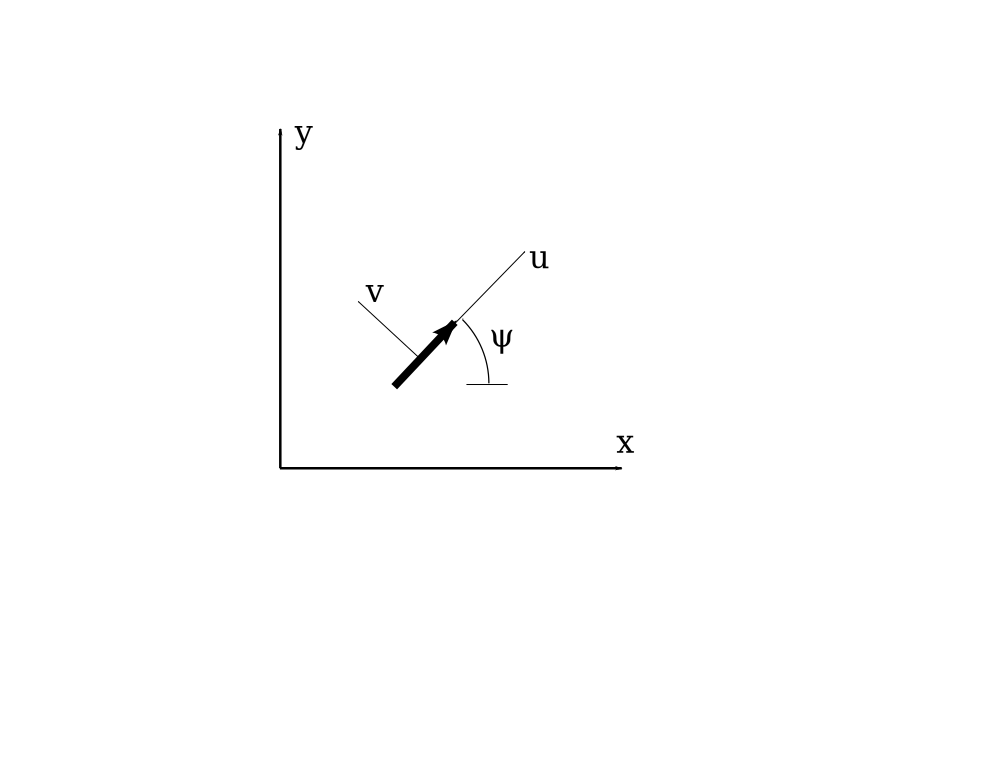
\includegraphics[width=\FigWidth\textwidth]{uni_model.png}
\caption{Illustration of the direct drive horizontal robot model.}
\label{f:uni_model}
\end{figure}

This model has three degrees of freedom; it can translate forward (the $u$ direction) and laterally (the $v$ direction) while rotating about the middle (the $\psi$ direction).  To describe this model we will use the following six states of the model, two inputs and five physical parameters.
\begin{itemize}
\item Model States
\begin{itemize}
\item $x$ and $y$: Position of the vehicle with respect to a fixed frame of reference.
\item $\psi$: Angular position of the vehicle relative to the $x$ axis.
\item $u$: Forward velocity of the vehicle with respect to the body-frame.
\item $v$: Lateral velocity of the vehicle with respect to the body-frame.
\item $r$: Angular velocity of the vehicle.
\end{itemize}
\item Inputs
\begin{itemize}
\item $F$: Force input in the forward direction with respect to the body-frame.
\item $T$: Torque input in the counter-clockwise direction.
\end{itemize}
\item Model Parameters
\begin{itemize}
\item $M$: Translational inertia (mass) of the vehicle
\item $I$: Rotational inertia (moment-of-inertia) of the vehicle
\item $d_u$: Translational damping/drag on the vehicle in the forward ($u$) direction
\item $d_v$: Translational damping/drag on the vehicle in the lateral ($v$) direction
\item $d_r$: Rotational damping/drag on the vehicle in the rotational ($\psi$) direction.
\end{itemize}
\end{itemize}

The equations of motion can be written as  a set of six, coupled, first-order differential equations.

\noindent
Kinematics:
\begin{eqnarray}\label{e:direct_kinematics}
\dot{x} & = & \cos{(\psi)}u - \sin{(\psi)}v \\
\dot{y} & = & \sin{(\psi)}u + \cos{(\psi)}v \\
\dot{\psi} & = & r
\end{eqnarray}

\noindent
Kinetics:
\begin{eqnarray}\label{e:direct_kinetics}
\dot{u} & = & -\frac{d_u}{M}u + \frac{1}{M}F \\
\dot{v} & = & -\frac{d_v}{M}v \\
\dot{r} & = & -\frac{d_r}{I}r + \frac{1}{I}T \\
\end{eqnarray}
If the damping factors ($d_u$, $d_v$ and $d_r$) are constants, this model represents linear drag behavior.
%This chapter is about \gls{robotmodel}s.

\begin{ex}
Derive the mathematical model in (\ref{e:direct_kinetics}) based on the physics of a rigid body moving on a plane.  A good place to start is with a free-body-diagram.
\end{ex}

\begin{ex}
Write a computational simulation of the motion described in (\ref{e:direct_kinematics}) and (\ref{e:direct_kinetics}) using the Euler numerical integration method described in Section~\ref{s:numerical}.  Start by writing on paper the discrete-time formulation of the model and then write a program/script that instantiates the dynamics.  Use the following model parameters:
\begin{itemize}
\item $M=\unit[10]{kg}$
\item $I=\unit[10]{kg m^2}$
\item $d_u=\unitfrac[5]{N}{m/s}$
\item $d_v=\unitfrac[25]{N}{m/s}$
\item $d_r=\unitfrac[4]{N}{rad/s}$
\end{itemize}

\noindent
The initial conditions are $x=y=0$ and $\psi = \unit[\pi/4]{rad}$.  

\noindent
Test your simulation by creating graphs of the position ($y$ versus $x$) as well as the angular position ($\psi$ versus time) for the following test inputs:
\begin{enumerate}
\item $F = \unit[10]{N}$ and $T = \unit[0]{Nm}$
\item $F = \unit[0]{N}$ and $T = \unit[1]{Nm}$
\item $F = \unit[10]{N}$ and $T = \unit[1]{Nm}$
\end{enumerate}


Note, you should be able to analytically predict the maximum (steady-state) tranlational and rotational velocities for this sytem.  This prediction will help you debug your simulation; if you know the analytical solution, you can determine if your simulation is 'working'.  You should also be able to predict the time constants associated with these first order equations.  This should give you some guidance about how small you will need to make $dt$ in your numerical integration.

Submit graphs that illustrate your numerical solution for the three test cases above.  These graphs should be discussed with brief text to clearly illustrate what you are trying to show.  Remember to use labels with units!

\end{ex}

\begin{ex}
Re-write the simulation described in the previous exercise, but write the numerical integration step as a function.  The function should have the following inputs:
\begin{itemize}
\item The current state of the robot as a 6 element vector at time $k$.
\item The current value for $F$
\item The current value for $T$
\item The size of the time-step $dt$
\end{itemize}
The function should return a 6 element vector for the new state at time $k+1$.

Now you should have a function for the Euler integration step (going from time $k$ to time $k+1$ AND a program that simulates the dynamics by moving through a set of discrete time steps.  Re-run the test cases in the previous exercise to validate your results.
\end{ex}


%\begin{ex}
%Choose a constant dt based on physical parameters
%\end{ex}

%\begin{ex}
%Write the simulation using some linear algebra
%\end{ex}

%\
%\begin{ex}
%Write an open-loop  controller
%Write a closed-loop controller - include a maximum force
%\end{ex}

\begin{ex}
A very similar standard model captures the dynamics of the same robot with two different inputs.  Figure~\ref{f:uni_model_diff} illustrates the same scenario as Figure~\ref{f:uni_model}, but, instead of a forward thrust and torque inputs, this model considers two, independent thrust inputs $F_L$ and $F_R$ separated by a distance of $2r$.

Re-write the equations (\ref{e:direct_kinematics} and (\ref{e:direct_kinetics}) for this new model.

\end{ex}

\begin{figure}[hbt]
\centering
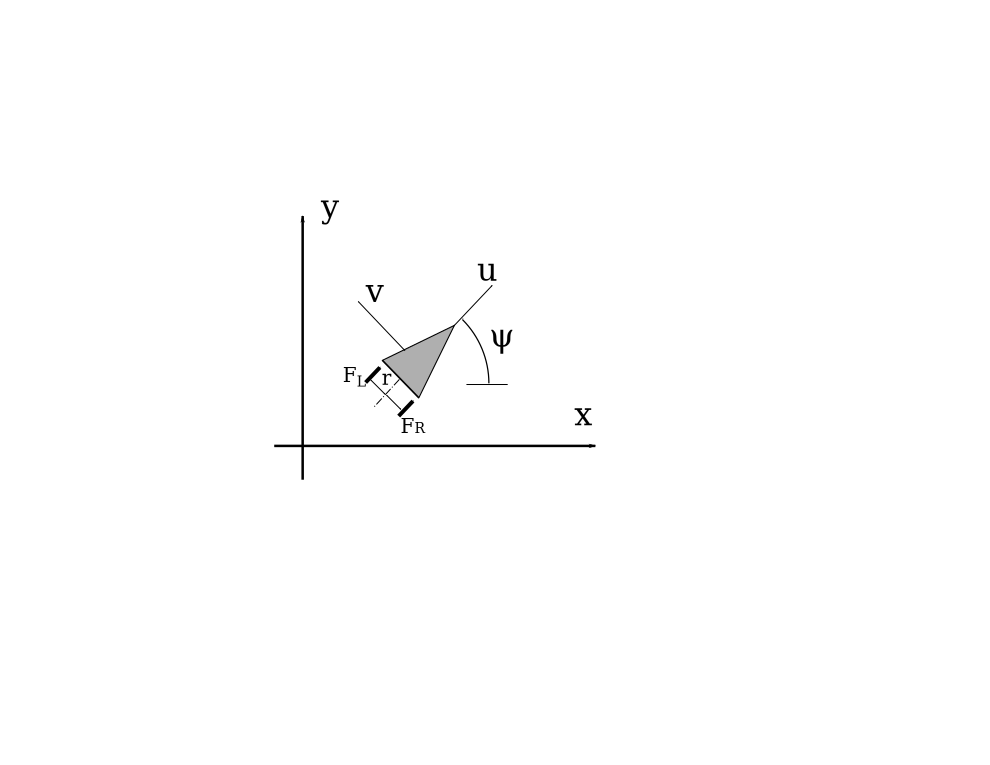
\includegraphics[width=\FigWidth\textwidth]{uni_model_diff.png}
\caption{Illustration of the differential drive variant of the horizontal robot model shown in Figure~\ref{f:uni_model}.}
\label{f:uni_model_diff}
\end{figure}
